\documentclass{article}
\usepackage[utf8]{inputenc}
\usepackage{graphicx}
\usepackage{hyperref}
\usepackage{amsmath}
\usepackage{amsfonts}
\usepackage{listings}
\usepackage{xcolor}
\graphicspath{ {./images/} }
\usepackage{natbib}
\usepackage{subfigure}
\usepackage[section]{placeins}

\definecolor{codegreen}{rgb}{0,0.6,0}
\definecolor{codegray}{rgb}{0.5,0.5,0.5}
\definecolor{codepurple}{rgb}{0.58,0,0.82}
\definecolor{backcolour}{rgb}{0.95,0.95,0.92}
\lstdefinestyle{mystyle}{
    backgroundcolor=\color{backcolour},   
    commentstyle=\color{codegreen},
    keywordstyle=\color{magenta},
    numberstyle=\tiny\color{codegray},
    stringstyle=\color{codepurple},
    basicstyle=\ttfamily\footnotesize,
    breakatwhitespace=false,         
    breaklines=true,                 
    captionpos=b,                    
    keepspaces=true,                 
    numbers=left,                    
    numbersep=5pt,                  
    showspaces=false,                
    showstringspaces=false,
    showtabs=false,                  
    tabsize=2
}

\lstset{style=mystyle}


\title{Entropy and Information in Lorenz Trajectories}


\begin{document}
\author{Daniele Noto}
\maketitle
\section{Lorenz '63 Model}
Lorenz's model is one of the first simplified model used to describe atmospheric convection. 
Here we can find the system of equation that defines it.
\begin{equation}
\left\{\ \begin{array}{l}
\dot{x}=\sigma(y-x) \\
\dot{y}=r x-y-x z \\
\dot{z}=x y-b z 
\end{array}\right.
\end{equation}
Where $\sigma$ is the Prandtl number, $r$ is the Rayleigh number and $b>0$ is a parameter linked to the ratio of the convective rolls.
With $\sigma=10$, $b=\frac{8}{3}$, $r=28$ the system will show a chaotic behaviour. [\citeyear{LorenzArticle}]

Given a dynamical system $\boldsymbol{\dot{x}}(t)=\boldsymbol{F}\big{(}\boldsymbol{x}(t)\big{)}$,  $\boldsymbol{x}^* \text{ is a fixed point if } \boldsymbol{F}(\boldsymbol{x}^*)=0.$ 
This system has three fixed points.

\begin{equation}
\begin{split}
    \boldsymbol{x}_0=&(0,0,0)\\
    \boldsymbol{x}_{1}=&\big{(}
    \p\sqrt{b(r-1)},\p\sqrt{b(r-1)},r-1 \big{)}\\
    \boldsymbol{x}_{2}=&\big{(} \m\sqrt{b(r-1)},\m\sqrt{b(r-1)},r-1 \big{)}\\
\end{split}
\end{equation}
The origin, $x_0$, is a fixed point for each possible value of the parameters while $\boldsymbol{x}^{*}_{1,2}$ exist only if $r>1$.
\subsection{Linear Stability Analysis of fixed points}
It is useful to study how the system behaves when it is close to one of its fixed point. We set $$\boldsymbol{x}(t)=\boldsymbol{x}^*+\boldsymbol{\eta}(t)$$
and we assume that $\boldsymbol{\eta}(t)$ is a small perturbation away $\boldsymbol{x}^*$. We substitute in $\dot{\boldsymbol{x}}(t)=\boldsymbol{F}(\boldsymbol{x}(t))$ and by neglecting terms in order $\boldsymbol{\eta}^2$ we obtain the evolution in time of the small perturbation.
\begin{equation}
    \boldsymbol{\dot{y}}(t)=\boldsymbol{A}\boldsymbol{y}
\end{equation}
Where $A = \frac{\partial \boldsymbol{F}(\boldsymbol{x}^*) }{\partial \boldsymbol{x}_{ij}}$ with eigenvalues $(\lambda_i)$. We say that $\boldsymbol{x}^*$ is linearly stable if $\Re(\lambda_i)\leq0$ $\forall i $ .
\paragraph{Stability of $\boldsymbol{x}^{*}_0$}
We can see that if we remove the non linearity the dynamics of $z(t)$ is decoupled. So we can analyse the evolution of only $x(t)$ and $y(t)$:
\begin{equation}
\left(\begin{array}{l}
\dot{x} \\
\dot{y}
\end{array}\right)=\left(\begin{array}{cc}
-\sigma & \sigma \\
r & -1
\end{array}\right)\left(\begin{array}{l}
x \\
y
\end{array}\right)
\end{equation}
The trace of the matrix is $\tau=-\sigma -1 <0$, and determinant $\Delta=\sigma(1-r)$.
$\boldsymbol{x}^{*}_0$ is unstable if $r>1$ ($\Delta<0$ and $\tau<0$ implies that $\lambda_i<0$ $ \forall i$).
\paragraph{Stability of $\boldsymbol{x}^{*}_{1,2}$}
These points exists only if $r>1$ and they are stable if: 
\begin{equation}
\begin{split}
    1<r<r_h=\frac{\sigma(\sigma+b+3)}{\sigma-b-1}\simeq27.4\\
\end{split}
\end{equation}
where $r_h$ is the critic value of $r$, i.e where the system begins to show its chaotic behaviour. 


\subsection{Analysis of Phase Space}
To compute the trajectories that has been used to study the phase space, the system has been solved numerically with RK4 method, with $\Delta t=0.01$. We analysed three different type of trajectories.
\begin{itemize}
    \item 9 trajectories, 3000 points length, with random initial condition. This set is denoted with $\mathcal{D}_{rnd}$.
    \item 9 trajectories, of 3000 points, that begin close to the three fixed points, three for each point. This set is denoted with $\mathcal{D}_{FP}$.
    %\item $\mathcal{D}_{rnd}=\{\boldsymbol{x}(t_k) \}_{k=1}^{N}$ with N=3000 sampled by a 27000 points trajectory.
    %\item $\mathcal{D}_{FP}=\{\boldsymbol{x}(t_k) \}_{k=1}^{N}$ N=3000, $\boldsymbol{x}(t_0)$ is close to one of the three fixed points
    %$\boldsymbol{x}^{*}_0,\boldsymbol{x}^{*}_1,\boldsymbol{x}^{*}_2$. 
    %\item We can split in three $\mathcal{D}_{FP}$, namely one dataset for each fixed point : $\mathcal{D}_{x_0}$, $\mathcal{D}_{x_1}$, $\mathcal{D}_{x_2}$
\end{itemize}
\begin{figure}[]
    \centering 
    \subfigure[]{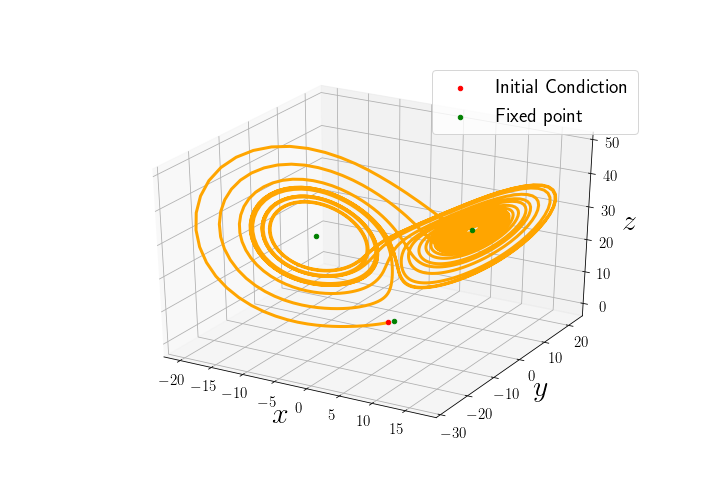
\includegraphics[width=\textwidth]{images/fixed_point_plot.png}}
    \subfigure[]{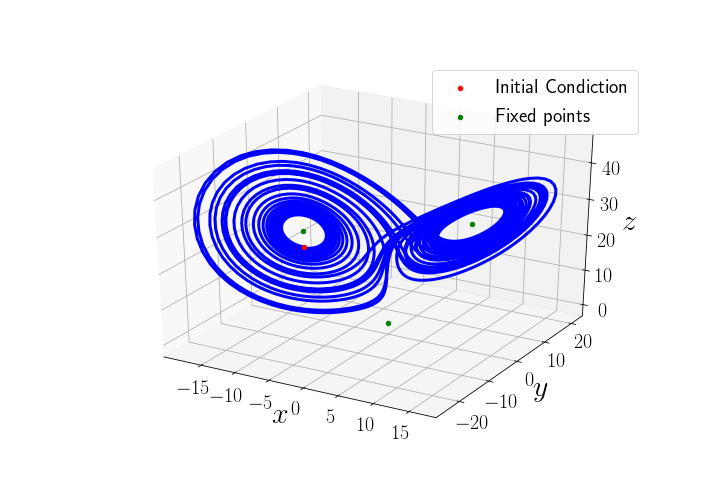
\includegraphics[width=\textwidth]{images/random_traj_plot.png}}
    \caption{(a)  Trajectory sample of $\mathcal{D}_{FP}$ (b) Trajectory sample of $\mathcal{D}_{rnd}$ }
    \label{fig:plot_traj}
\end{figure}
In Fig.\ref{fig:plot_traj} we see two sample of the two sets of trajectories.

As it has been shown in [\citeyear{bucci2021leveraging}], although the fixed and the random trajectories have the same amount of data, the performances of a Neural Network (LSTM) are better if the training is $\mathcal{D}_{FP}$ rather than the $\mathcal{D}_{rnd}$. 
\subsection{$S_{svd}$}
The amount of information that a trajectory contains, according to the Information Theory, is the minimum number of bit needed to reproduce it entirely.[\citeyear{shannonEntropy}]

To measure it we used the $S_{svd}$ that it is based on Single Value Decomposition (known also as Principal Component Analysis [\citeyear{PCA}]) a method that has been widely used in different fields, ,[\citeyear{TamingChaos}].
We can define it as following:
\begin{equation}
    S_{svd}=S(\mathbf{x}(t),order,delay)
\end{equation}
We denote with $\mathbf{x}(t)$ the dataset that we want to study. 
\begin{equation}
\begin{split}
    &\mathbf{x}(t_0)=x_{0},\\
    &\mathbf{x}(t)=(x_1,x_2,x_3,\ldots,x_N)
\end{split}
\end{equation}
This function creates a matrix Y with the dataset.
\begin{equation}
\begin{split}
    \mathbf{y}(i)=(x_i,x_{i+\text{delay}}, ...,x_{i+(\text{order}-1)\text{delay}})
\end{split}
\end{equation}
\begin{equation*}
    Y = 
\begin{pmatrix}
\mathbf{y}(1) \\
\mathbf{y}(2) \\
. \\
. \\
. \\
\mathbf{y}(N-(ord-1)del)
\end{pmatrix}
\end{equation*}
If we use $order=3$ and $delay=1$ we obtain the following matrix:

\begin{equation*}
    Y = 
\begin{pmatrix}
x_1 & x_2 & x_3 \\
x_2 & x_3 & x_4 \\
. & . & .\\
. & . & .\\
. & . & .\\
. & x_{N-1} & x_N \\
\end{pmatrix}
\end{equation*}
The next step is to apply SVD decomposition to the matrix Y.
\begin{equation}
    Y=U\Sigma V^{*}
\end{equation}
Where U is an unitary matrix, V is also an unitary matrix, and $\Sigma$ is a diagonal matrix.
We denotes the eigenvalues of the matrix $\Sigma$ with $\sigma_i$. After we compute the average eigenvalues:
\begin{equation}
    \bar{\sigma}_k=\frac{\sigma_k}{\sum_j^M\sigma_j} 
\end{equation}
Where M is the number of eigenvalues.

After this we can compute the SVD Entropy:
\begin{equation}
    S_{svd}=-\sum^{M}_{k}\bar{\sigma}_k log_2(\bar{\sigma}_k)
\end{equation}

\begin{figure}[h]
    \centering
    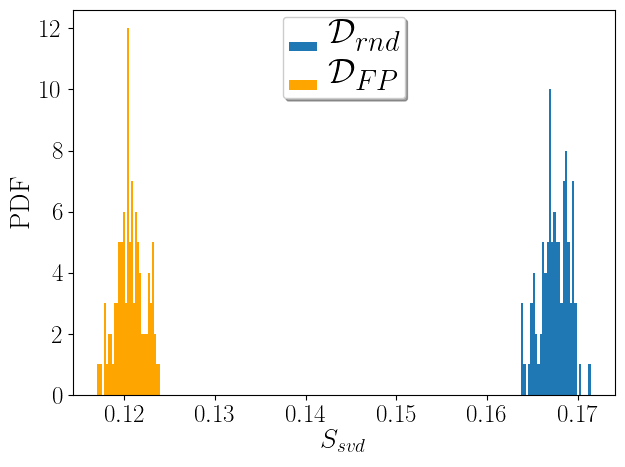
\includegraphics[width=0.7\textwidth]{images/entropy_svd_fixed_vs_random.png} 
    \caption{Histogram of $S_{svd}$ of 100 trajectories for each type of dataset. It is shown that the fixed point dataset has less entropy}
    \label{fig:histogram_entropy}
\end{figure}
\begin{figure}
    \centering
    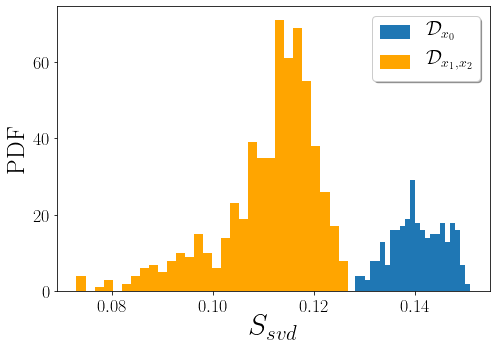
\includegraphics[width=0.7\textwidth]{images/entropy_svd_zeroVSother.png}
    \caption{$S_{svd}$ histogram of $\mathcal{D}_{x_{0,1,2}}$ trajectories, 300 for each fixed point. We can see that the $\mathcal{D}_{x_0}$ has more entropy}
    \label{fig:SVD-Entropy_statistic_012}

\end{figure}
In figure \ref{fig:histogram_entropy} we have computed the average $S_{svd}$ for 100 samples of 9 trajectories of $\mathcal{D}_{rnd}$ and $\mathcal{D}_{FP}$.

\subsection{$S_{svd}$ analysis of trajectories}
We can study the $\mathcal{S}_{svd}$ of the trajectories to see how it grows increasing the number of points.
\begin{figure}[h]
    \subfigure[]{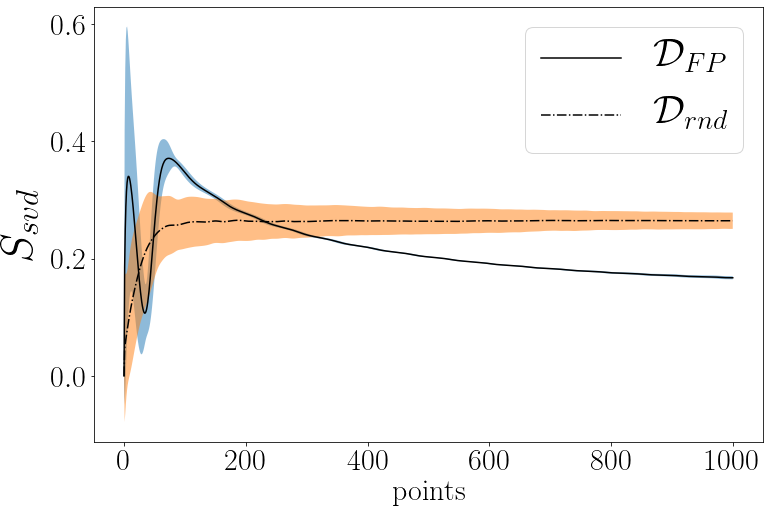
\includegraphics[width=0.5\textwidth]{images/SVDEntropyFixed_vs_Random_long.png}}
    \subfigure[]{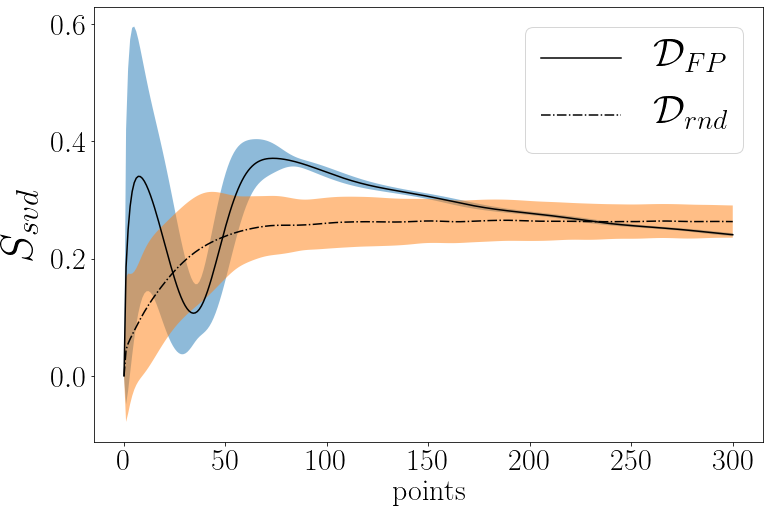
\includegraphics[width=0.5\textwidth]{images/SVDEntropyFixed_vs_Random_short.png}}
    \caption{(a) Average $S_{svd}$ of 100 trajectories with its fluctuation (1 std) (b) Zoom on the first 300 points of $S_{svd}$}
    \label{fig:SVD-Entropy_statistic}
\end{figure}
In Fig \ref{fig:SVD-Entropy_statistic} it has been shown the close to 200 number of points we can see that the amount of $S_{svd}$ is bigger in the random trajectories.
Fixed points trajectory shows to have less variance than the random one, except for the first 100 points, that shows higher fluctuations.
To see what is the cause of higher fluctuations we can study the $S_{svd}$ of trajectories close to $\boldsymbol{x}^{*}_{0,1,2}$ separately.

\begin{figure}
    \subfigure[]{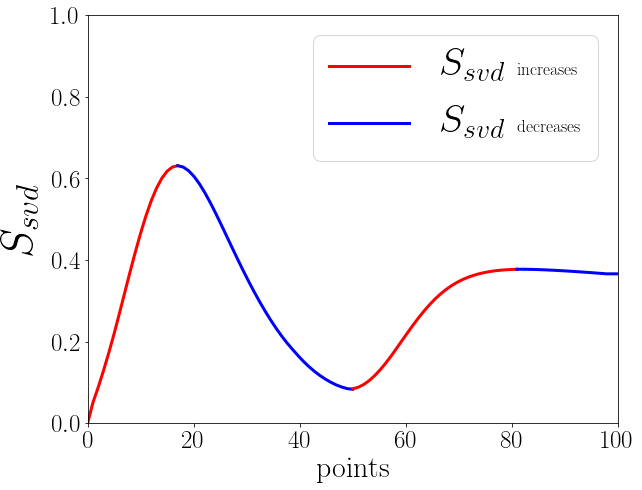
\includegraphics[width=0.5\textwidth]{images/IncreaseDecrease_SVD-Entropy.png}}
    \subfigure[]{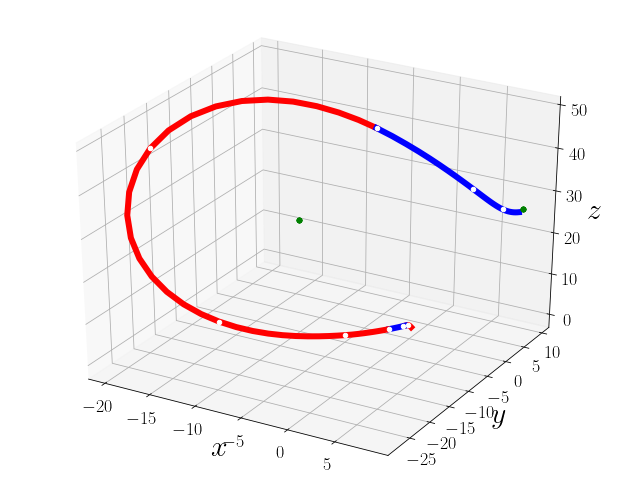
\includegraphics[width=0.5\textwidth]{images/Lorenz_Trajectory_step_zero.png}}\\
    \subfigure[]{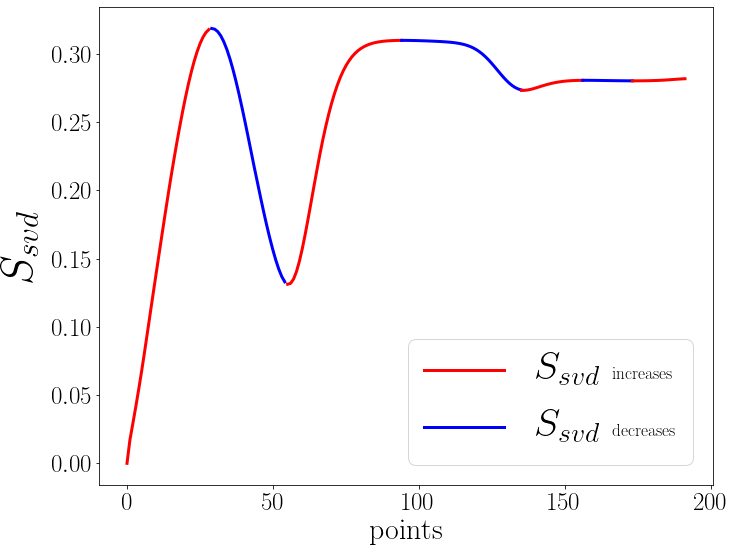
\includegraphics[width=0.5\textwidth]{images/IncreaseDecrease_SVD-Entropy-rnd.png}}
    \subfigure[]{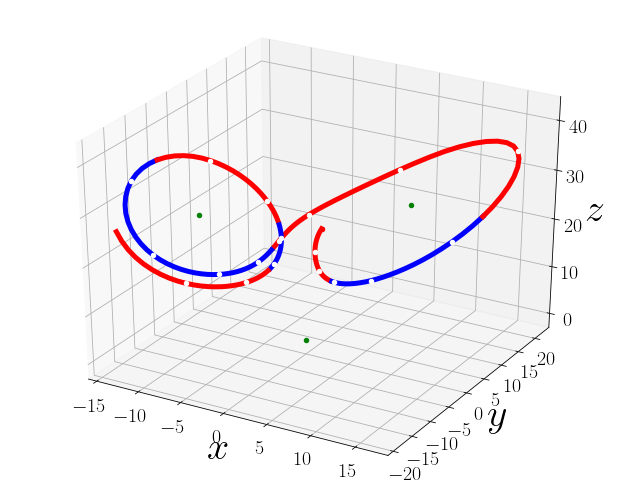
\includegraphics[width=0.5\textwidth]{images/lorenztraj_svd_growth.png}}\\
    
    \caption{(a) Evaluation of the $S_{svd}$ of the trajectory $\mathcal{D}_{x_{0}}$ (b) Trajectory from $\mathcal{D}_{x_0}$ the white points are plotted every 10 time steps (c) $S_{svd}$ of the trajectory in (d) sampled from $\mathcal{D}_{rnd}$}
    \label{fig:growth_svd}

\end{figure}

We have evaluated the $S_{svd}$ for $\mathcal{D}_{x_{0,1,2}}$, by taking 300 trajectories for each set, to show the difference in entropy between $\mathcal{D}_{x_0}$ and $\mathcal{D}_{x_{1,2}}$ . In Fig. \ref{fig:SVD-Entropy_statistic_012}, we can see the fluctuation that has been noticed in Fig. \ref{fig:SVD-Entropy_statistic} are caused by the trajectories of $\mathcal{D}_{{x}_0}$. 
\begin{figure}
    \centering 
    \subfigure[]{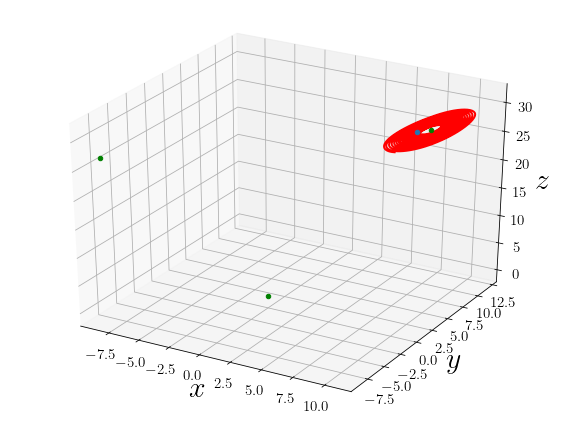
\includegraphics[width=0.7\textwidth]{images/Lorenz_Trajectory_others.png}}
    \subfigure[]{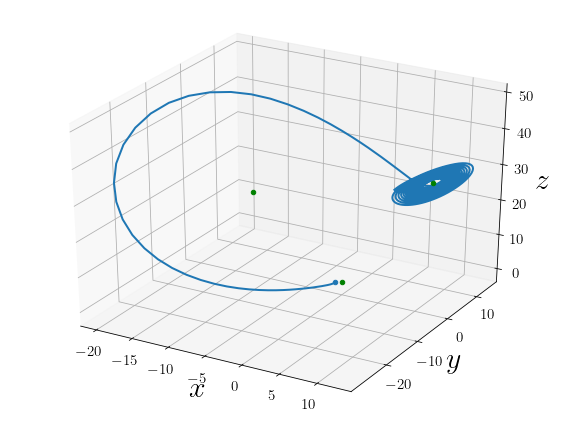
\includegraphics[width=0.7\textwidth]{images/Lorenz_Trajectory_zeros.png}}
    \caption{(a) Trajectory sampled from $\mathcal{D}_{x_1}$ (b) Trajectory sampled from $\mathcal{D}_{x_0}$  }
    \label{fig:different_trajectories}
\end{figure}
This difference is given by the fact that the trajectories of $\mathcal{D}_{x_0}$ are different from $\mathcal{D}_{x_{1,2}}$. At the begin $\boldsymbol{x}^{*}_0$ moves in a large space in the attractor, and faster than $\boldsymbol{x}^{*}_{1,2}$ ( see Fig.\ref{fig:different_trajectories} ). After almost 80 timesteps the trajectory moves to $\boldsymbol{x}_{1}$ or $\boldsymbol{x}_{2}$. It is observed in Fig. \ref{fig:growth_svd} [(a) and (b)], in which we can see the trajectory and how the $S_{svd}$ changes when it reaches different section of the phase space. 
When it is close to the two fixed points the fluctuations start to decrease. 



To be more confident with our results we can also repeat this analysis using, instead of $S_{svd}$ the Fisher Information, (see Appendix), and we obtain the same results.

\newpage
\section{Machine Learning Approach}
After we have showed, just analysing the trajectories, that the set $\mathcal{D}_{FP}$ is the most informative, we can develop a Machine Learning model and analyse it during the training process. We are going to determinate the amount of information that it is extracted by the models from each dataset.
\section{Models and Methods}
We used two models to learn the Lorenz Model.
\subsection{RNN}
The first model is a standard RNN [\cite{rumelhart:errorpropnonote}] with the following parameters:
\begin{itemize}
    \item 1 layer is an RNN 
    \item 2 layer is linear layer with in-features=50 out-features=3
\end{itemize}

\subsection{MLP}
The model that is used for training is a Multy Layer Perceptron [\citeyear{Rosenblatt58theperceptron:}], with 3 layers:
\begin{itemize}
  \item (layer 1): Linear(in-features=3, out-features=60)
  \item (layer 2): Linear(in-features=60, out-features=42)
  \item (layer 3): Linear(in-features=42, out-features=3)
\end{itemize}
With ReLU as activation functions.
\begin{figure}[h]
    \centering
    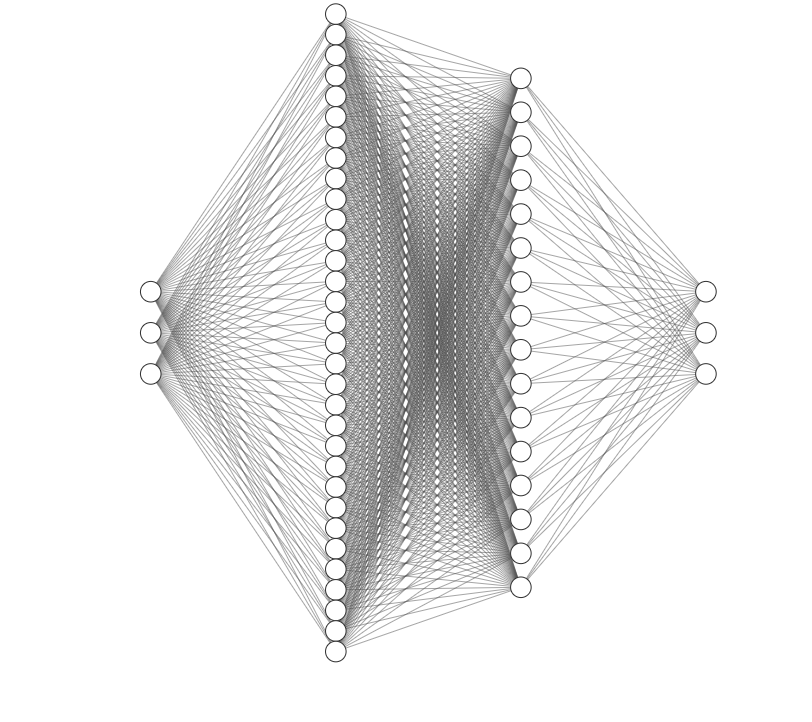
\includegraphics[width=0.8\textwidth]{images/MLP.png}
    \caption{View of architecture of the MLP }
    \label{fig:MLP}
\end{figure}

\subsection{Fisher Information Matrix}
Given a dataset $\mathcal{D}$ we want to study the amount of information that a machine learning model extracts from it during the training process. To measure this quantity we use the Fisher Information Matrix [\citeyear{FIM}]. 

Given a dataset $\mathcal{D}=\{x_i\}^{N}_{i=1}$ with $x \sim f(x|\theta)$, and $\hat{\theta}$ an estimator of $\theta$:
The theorem of Cramer-Rao says that:
\begin{equation}
     \mathbb{E}[(\theta-\hat{\theta})^2]\geq \frac{1}{n \mathbb{E}\big{[}(\frac{\partial}{\partial \theta}\log f(x|\theta))^2\big{]}}
\end{equation}
We can denote as the Fisher Information, the denominator of this equation. As the theorem says, the Fisher Information give an esteem of how far is the predicted parameter to the real one.
\begin{equation}
    \mathcal{I}(\theta) := n \mathbb{E}_{\theta}\Big{[}\Big{(}\frac{\partial}{\partial \theta}\log f(x|\theta)\Big{)}^2\Big{]}
\end{equation}
If the distribution $f$ is a function of more than one parameter, $\boldsymbol{\theta}$,  we can write the Fisher Information Matrix as follows.
\begin{equation}
    I(\boldsymbol{\theta}) := \mathbb{E}_{\boldsymbol{\theta}}\left[\left(\boldsymbol{\nabla}_{\boldsymbol{\theta}} \log f(\mathbf{x} ; \boldsymbol{\theta})\right)^{2}\right]
\end{equation}
The eigenvalues of this matrix show the most informative directions in parameter space.
In practise we use the loss function as likelihood (MS2-error):

\begin{equation}
    \mathcal{L}_{i}=\left\|\boldsymbol{x}_{i}-{f}\left(\mathbf{x}_{i} ; \boldsymbol{\theta}\right)\right\|_{2}^{2}
\end{equation}
\begin{equation}
    \widehat{f}\left(\widehat{\mathbf{x}}_{i} ; \boldsymbol{\theta}\right)=\frac{\exp \left(-\mathcal{L}_{i} / \sigma^{2}\right)}{N^{-1} \sum_{j=1}^{N} \exp \left(-\mathcal{L}_{j} / \sigma^{2}\right)}
\end{equation}
\begin{equation}
    \boldsymbol{\nabla}_{\boldsymbol{\theta}} \log f\left(\widehat{\mathbf{x}}_{i} ; \boldsymbol{\theta}\right) \sim-\boldsymbol{\nabla}_{\boldsymbol{\theta}} \mathcal{L}_{i}+\frac{\sum_{k} \exp \left(-\mathcal{L}_{k} / \sigma^{2}\right) \boldsymbol{\nabla}_{\boldsymbol{\theta}} \mathcal{L}_{k}}{\sum_{j} \exp \left(-\mathcal{L}_{j} / \sigma^{2}\right)}
    \label{pratical_FIM}
\end{equation}
At the end the idea is to compute the (\ref{pratical_FIM}) at the begin and after 200 epochs, to measure how the model extracts information from each dataset.

\subsection{Results of Learning analysis}

\begin{figure}[h]
    \centering
    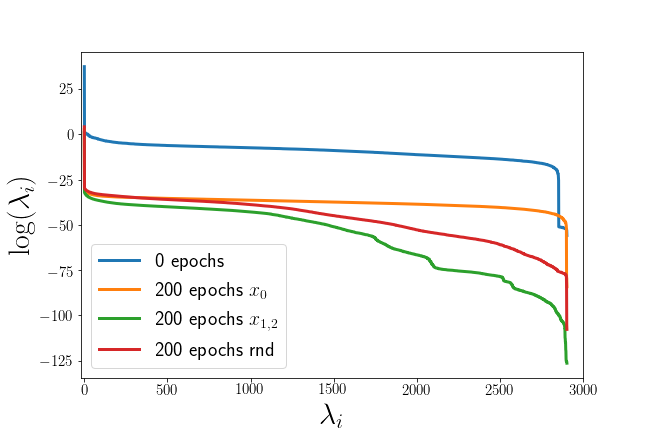
\includegraphics[width=0.8\textwidth]{images/FIM_different_fixed_points_rand.png}
    
    \caption{Fisher Information Matrix, spectrum of the norm of the eigenvalues, for RNN trained with $\mathcal{D}_{x_{0}},\mathcal{D}_{x_{1}},\mathcal{D}_{x_{2}},\mathcal{D}_{rnd}$. The model that extracts more information is the one who has been trained with $\mathcal{D}_{x_{1,2}}$}
    \label{fig:FIM_RNN}
\end{figure}
As we can see in Fig. \ref{fig:FIM_RNN} we can see that the eigenvalues are smaller in the model trained with $\mathcal{D}_{x_{1,2}}$ than the one with $\mathcal{D}_{x_0}$ or $\mathcal{D}_{rnd}$. This means that the model extracts more information if the dataset is made of trajectories that lies close to fixed points for the majority of the time.

\begin{figure}[h]
    \centering
    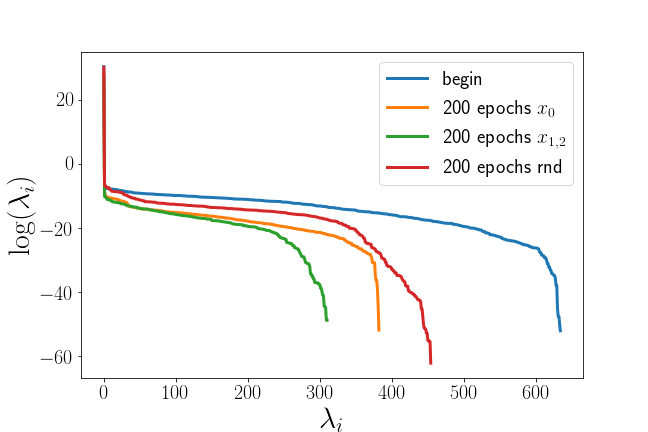
\includegraphics[width=0.8\textwidth]{images/FIM_MLP700_fixedVSrandom_0_200ep.png}
    \caption{We can see that the model trained with $\mathcal{D}_{x_{1,2}}$ extracts more information than the others}
    \label{fig:MLP_points}
\end{figure}

\section{Conclusion}

It has been shown, by following two parallel approaches that the dataset made of trajectories that are close to fixed points, $\mathcal{D}_{FP}$, is the most informative one. It is shown also that there is a significant difference between $\mathcal{D}_{x_0}$ and $\mathcal{D}_{x_{1,2}}$ if we talk about the amount of information that the model is able to extract. We shown that the dataset $\mathcal{D}_{x_{1,2}}$ is the one that contains more information.




\newpage
\section{Appendix}
%\noindent
%\includegraphics[width=0.5\textwidth]{images/fisher_info_long_traj.png}
%\includegraphics[width=0.5\textwidth]{images/long_short_FisherInfo_traj.png}\\
\subsection{Fisher Information}
Fisher information is used together with svd decomposition.
We can define the Fisher Information in the following way [\cite{TamingChaos}] :
\begin{equation}
    I_{F}=\sum^{M-1}_{k}\frac{(\bar{\sigma}_{k+1}-\bar{\sigma}_{k})^2}{\bar{\sigma}_{k-1}}
\end{equation}
The notation is the same that we have in $S_{svd}$. This represents the information that a trajectory contains, and it increases when the $S_{svd}$ decreases.
\begin{figure}
    \centering
    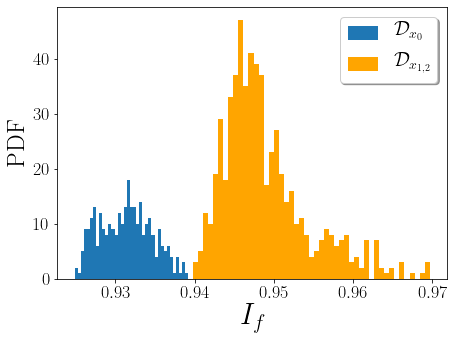
\includegraphics[width=0.6\textwidth]{images/fisher_info_ZeroVSother.png}
    \caption{Histogram of Fisher Information of 300 trajectories for each fixed point, sampled by $\mathcal{D}_{x_0}$ and $\mathcal{D}_{x_{1,2}}$. }
    \label{fig:fisher_histogram_0vs12}
\end{figure}
In Fig. \ref{fig:fisher_histogram_0vs12} we have the analogous plot of Fig. \ref{fig:SVD-Entropy_statistic_012}, the only difference is that in this case instead we measure the Fisher Information.

\nocite{*}
\bibliographystyle{mnras}
\bibliography{biblio}

\end{document}
